\section{Data and preparation}\label{ch:data}

This section identifies the ECG sources, explains how the signals are
prepared, and shows how examples enter model fitting, validation, and the
temporal test. Keeping these roles separate prevents healthy data or test
labels from being used in the wrong part of the study.

\subsection{Data sources and roles}

Two public PhysioNet databases supply model development data. A separate,
limited external INCART check is reported in the results chapter. The MIT--BIH Normal Sinus Rhythm
Database (NSRDB) supplies normal-reference ECG for the autoencoder. The MIT--BIH
Arrhythmia Database (MITDB) supplies labelled normal and abnormal beats for the
detector, subtype classifier, and final temporal evaluation
\cite{goldberger2000physionet,nsrdb,mitdb}.

\begin{table}[H]
\centering
\small
\caption{Data sources and their strictly separated roles.}
\label{tab:data-source-role}
\begin{tabular}{@{}>{\raggedright\arraybackslash}p{2.6cm}>{\raggedright\arraybackslash}p{3.8cm}>{\raggedright\arraybackslash}p{4.8cm}@{}}
\toprule
Source & Available data & Use in this study\\
\midrule
\makecell[l]{MIT--BIH\\Normal Sinus\\Rhythm DB\\(NSRDB)} &
18 real long-term ECG recordings from five men aged 26--45 and 13 women aged
20--50, with no significant arrhythmias; two stored channels named ECG1 and
ECG2; 128 Hz; approximately 23--26 hours per record \cite{nsrdb}. &
The complete first stored ECG channel from every record is processed. Fifteen
subjects fit the normal-only autoencoder and three different subjects validate
it and determine the normal residual threshold.\\
\addlinespace
\makecell[l]{MIT--BIH\\Arrhythmia DB\\(MITDB)} &
48 approximately 30-minute, two-channel ambulatory ECG records from 47
subjects (25 men aged 32--89 and 22 women aged 23--89), sampled at 360 Hz,
with expert beat and rhythm annotations \cite{mitdb,moody2001impact}. &
Only the 46 records containing MLII are eligible. Their earlier 80\% supplies
supervised development and their final 20\% supplies the temporal test. These
records represent 45 subject clusters because records 201 and 202 belong to
one person.\\
\bottomrule
\end{tabular}
\end{table}

Figure~\ref{fig:data-source-overview} summarises these roles. NSRDB supplies
normal-reference windows for the autoencoder, while MITDB supplies labelled
MLII beats for supervised development and temporal testing.

\begin{figure}[H]
\centering
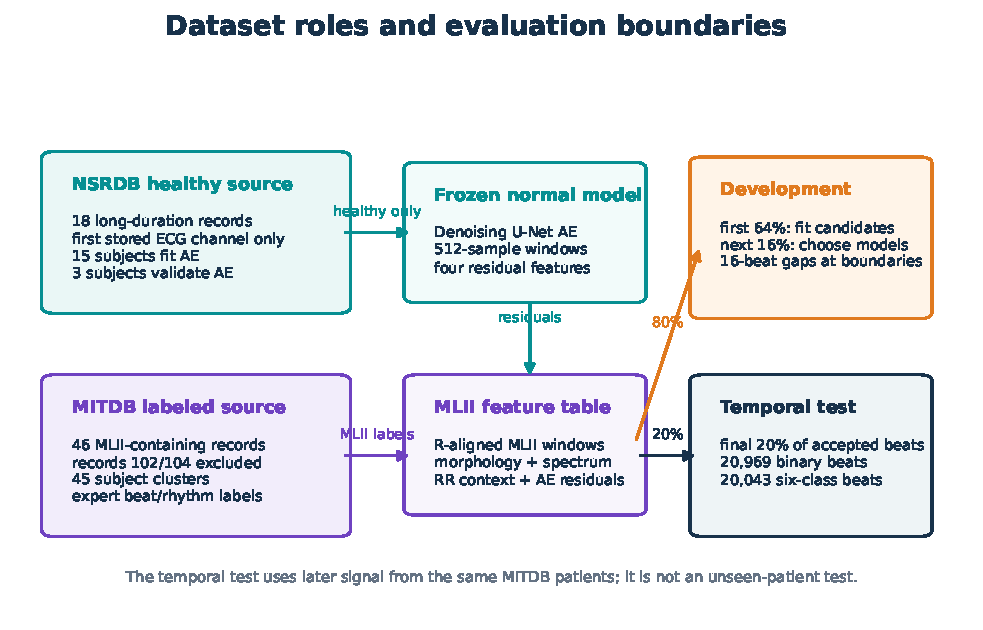
\includegraphics[width=.98\textwidth]{pic/generated/dataset_role_overview.pdf}
\caption{Dataset roles and evaluation boundaries. The healthy NSRDB channel
creates the frozen normal model. MITDB MLII creates the supervised feature table
and is split chronologically into development and temporal-test regions.}
\label{fig:data-source-overview}
\end{figure}

\textbf{Why NSRDB is used for healthy training.}
NSRDB contains real long-duration ECG from subjects reported to have no
significant arrhythmias. This matches the autoencoder idea: the network sees
normal structure without supervised arrhythmia labels. This is a nominally
normal source cohort, not an annotation-verified guarantee that every window
is normal. The preparation code does not exclude windows using NSRDB beat
annotations. All 18 subjects
and their complete recordings enter the cleaning process, giving 437.49 hours
of source ECG. Complete recordings also expose the model to normal within-day
variation instead of a short selected excerpt.

\textbf{Exactly one channel is used.}
NSRDB headers call the two waveforms ECG1 and ECG2; they do not identify either
as a standard anatomical lead. This study therefore selects the first stored
channel consistently and describes it as the \emph{first NSRDB ECG channel}.
It is not renamed Lead II. The second channel never enters autoencoder fitting,
validation, threshold estimation, or residual calculation.

The supervised branch uses MLII only. Modified Lead II is a bipolar torso
lead with a negative RA-equivalent electrode on the right upper torso and a
positive LL-equivalent electrode on the left lower torso. Figure~\ref{fig:data-lead-positions}
shows this polarity schematically; the separate reference electrode is shown
for the project's sensor connection. It does not represent a second ECG
channel. PhysioNet describes the modified torso lead and its generally
prominent normal QRS complexes \cite{physionetLeadFAQ,mitdb}. The
loader selects MLII by its header name rather than assuming a channel number.
MLII is stored first in 45 eligible records; record 114 stores V5 first and
MLII second. Records 102 and 104 contain V5 and V2 but no MLII and are
excluded. Consequently, the detector, classifier, temporal test, and installed
replay all receive one MLII waveform.

Both data streams contain one channel, but their lead identities differ: the autoencoder learns healthy structure
from the first NSRDB channel, while the supervised hierarchy operates on MLII.
This source difference is a limitation because the electrode placement for the
NSRDB channel is not documented.

\begin{figure}[H]
\centering
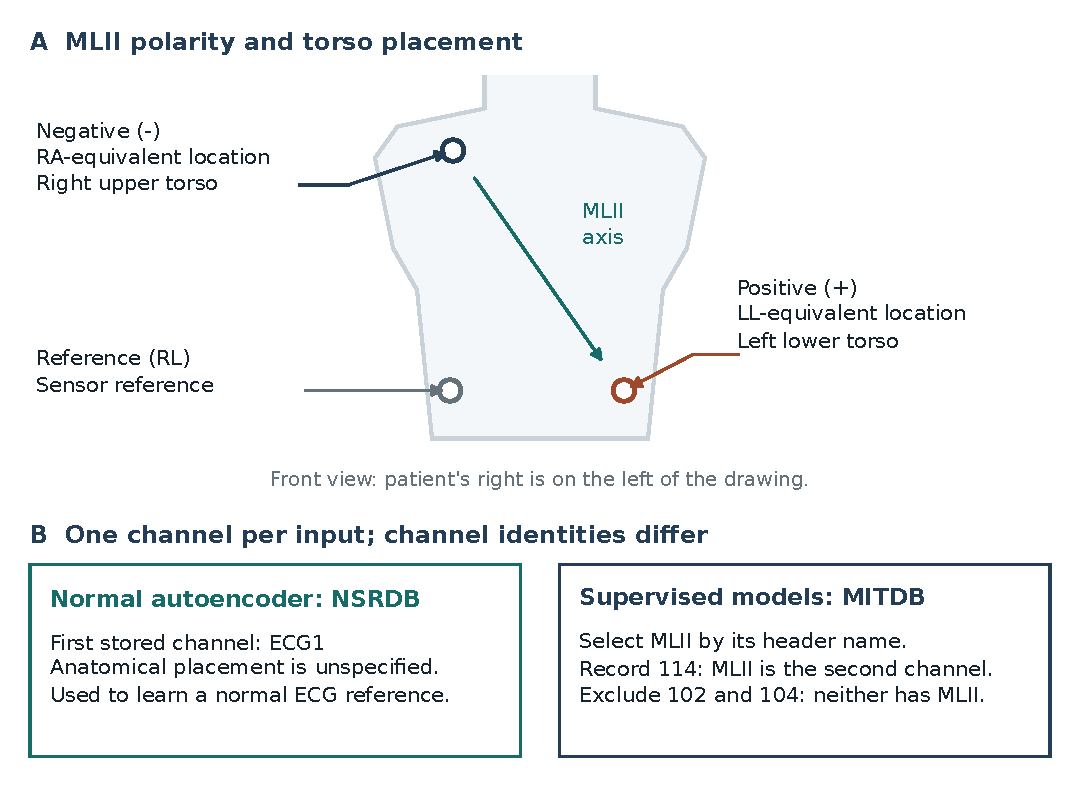
\includegraphics[width=.98\textwidth]{pic/generated/real_lead_positions.pdf}
\caption[MLII polarity and the channel used by each model.]{MLII polarity and
the channel used by each model. Panel A is an anterior-view schematic of the
modified Lead-II axis, with the project's reference connection shown separately;
it is not an exact map of the database electrode coordinates
\cite{physionetLeadFAQ}. Panel B distinguishes the NSRDB ECG1 normal reference
from the MLII input used by the supervised models.}
\label{fig:data-lead-positions}
\end{figure}

\textbf{Reference labels.}
MITDB expert annotations are mapped to the six project outputs as shown in
Table~\ref{tab:data-label-map}. AFib is determined from the rhythm annotation
around a beat; the other targets mainly use beat symbols.

\begin{table}[H]
\centering
\small
\caption{Mapping from MITDB expert annotations to project outputs.}
\label{tab:data-label-map}
\begin{tabular}{lll}
\toprule
Output & MITDB evidence & Interpretation\\
\midrule
N & N, e, j outside AFib/AFL & normal-like/escape group\\
PVC & V, E & ventricular premature or escape beat\\
PAC & A, a, J, S & supraventricular premature beat\\
LBBB & L & left bundle branch block beat\\
RBBB & R & right bundle branch block beat\\
AFib & normal-like beat inside AFIB/AFL rhythm & atrial fibrillation/flutter context\\
\bottomrule
\end{tabular}
\end{table}

The class codes are project groupings, not exact clinical diagnoses or the
standard AAMI five-class scheme. N includes atrial and junctional escape beats;
PVC includes ventricular escape beats; PAC includes nodal and supraventricular
premature beats. AFib combines fibrillation and flutter rhythm annotations
only when the beat symbol maps to N. Other supported beat types retain their
morphology label during AFIB/AFL. Consequently, AFib recall here is neither
pure AF sensitivity nor episode-level AF detection.

Unsupported symbols remain abnormal in binary evaluation and are excluded
from six-class scoring. At runtime, a gated unsupported abnormality still
receives one of the five available subtype labels. The prepared MLII dataset contains 104,755 accepted beats: 63,073
in group N and 41,682 abnormal. Of these, 100,072 have a supported six-class label.

\subsection{Signal cleaning and window construction}

Data preparation converts the two ECG sources into a common input shape: one four-second signal with 512 samples. The supervised preparation rules were fixed for the rerun and are also used
during session prediction. NSRDB retains its original preparation procedure.
Figure~\ref{fig:data-cleaning-real} shows the full transformation for one
healthy NSRDB segment and one MITDB MLII beat.

\subsubsection{Cleaning checks}

Table~\ref{tab:data-cleaning-checklist} lists the preparation steps and their
purpose. Rejected windows do not enter model fitting or evaluation.

\begin{table}[H]
\centering
\small
\caption{Cleaning checklist applied before a signal can become a model input.}
\label{tab:data-cleaning-checklist}
\begin{tabular}{>{\raggedright\arraybackslash}p{2.6cm}>{\raggedright\arraybackslash}p{5.0cm}>{\raggedright\arraybackslash}p{4.3cm}}
\toprule
Step & What is done & Why it matters\\
\midrule
Required channel & NSRDB must provide ECG1; MITDB must provide MLII. Missing
required signals stop processing. & Prevents accidental use of ECG2, V5, V2, or
another non-matching lead.\\
\addlinespace
Sampling rate & NSRDB remains at 128 Hz. MITDB MLII is resampled from 360 Hz to
128 Hz with polyphase anti-aliasing. & Makes every four-second model window
exactly 512 samples.\\
\addlinespace
Band-pass filter & A Butterworth band-pass with prototype order four
and cutoffs 0.5--50 Hz uses forward--backward filtering. For supervised inputs
this is applied within the four-second window \cite{butterworth1930filter,virtanen2020scipy}. & Reduces baseline drift and high-frequency noise while avoiding filter-induced
phase delay.\\
\addlinespace
Amplitude standardisation & Each supervised MLII window is converted to approximately zero mean
and unit standard deviation; NSRDB retains its archived scaling. & Reduces gain differences while preserving the
relative P--QRS--T shape.\\
\addlinespace
Window quality check & Corrected supervised windows must be finite and
non-flat. Both neighbouring R peaks must be observed. & Rejects unusable
inputs. These checks do not establish clinical signal quality or remove all
motion artifacts.\\
\bottomrule
\end{tabular}
\end{table}

\subsubsection{Window construction}

The autoencoder and supervised hierarchy build windows in different ways, but
the final array shape is the same. The autoencoder receives consecutive,
non-overlapping four-second windows from the first stored NSRDB channel. The
supervised MLII windows are aligned to a beat: 200 samples before the R peak
and 312 samples starting at the R peak. During offline experiments, expert annotations give
the R-peak location for alignment and later scoring. During live use, detected
R peaks replace those annotations.

For samples $x_1,\ldots,x_n$ inside one prepared model window, amplitude
standardisation is
\begin{equation}
 z_i=\frac{x_i-\mu}{\sigma+10^{-8}},\qquad
 \mu=\frac{1}{n}\sum_{i=1}^{n}x_i.
\end{equation}
The corrected supervised pipeline filters each extracted window and applies
this operation locally. The original experiment instead standardised each
complete MITDB record before extracting windows. That used test-region signal
statistics during preparation and differed from sensor chunks. The results reported here use the local
preparation procedure. NSRDB remains the frozen
reference checkpoint with its archived input scaling. The real-data audit in
Section~\ref{sec:method-real-case} shows that an archived NSRDB window is not
unit variance; the current cache-building code must not be treated as proof
of the older cache's normalisation.

\subsubsection{Cleaning yield}

The healthy NSRDB recordings produce many candidate windows because complete
records are used instead of short excerpts. Across the 18 complete NSRDB
records, 393,744 candidate windows were formed. The quality checks kept 345,850
windows and rejected 47,894. These accepted windows were then split into
288,673 autoencoder fitting windows and 57,177 validation windows.

MITDB cleaning produces beat-aligned MLII examples. The prepared MLII dataset
contains 104,755 beats: 63,073 in group N and 41,682 abnormal. Unsupported abnormal
symbols are still used for binary abnormality evaluation, but they are excluded
from six-class subtype scoring.

\subsubsection{Preparation during prediction}

The corrected hierarchy applies the same local window filtering,
standardisation and feature order during fitting, offline scoring and
installed use. Database replay first resamples the signal. Sensor acquisition
supplies 128 Hz samples. Labels never enter a prediction.
The live backend waits until there is enough signal around a detected R peak
and enough RR context. It then feeds one prepared MLII window to the frozen
system. Neither supervised model is retrained during prediction.

\begin{figure}[H]
\centering
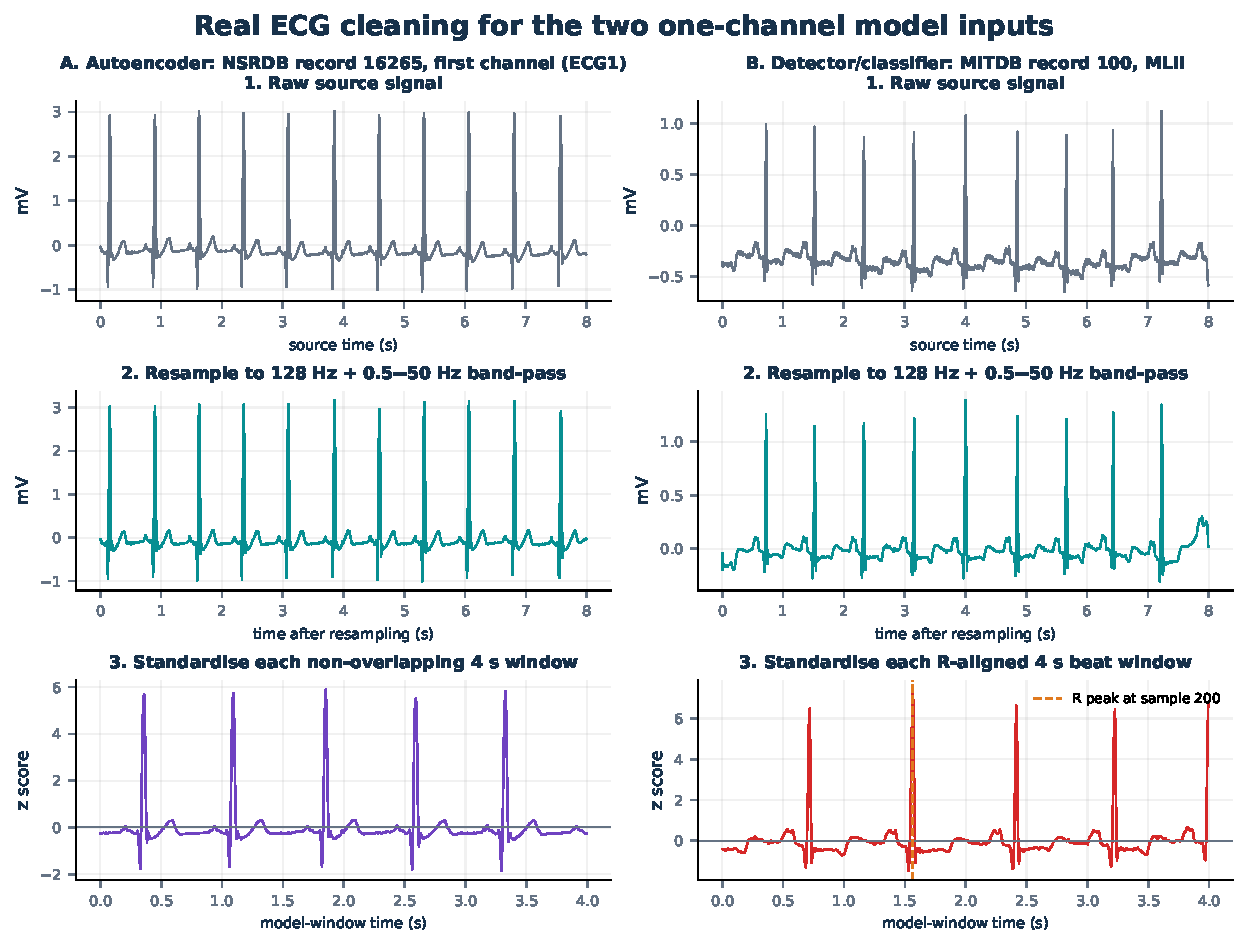
\includegraphics[width=.96\textwidth]{pic/generated/real_data_cleaning_pipeline.pdf}
\caption{Cleaning real ECG for the two roles. The normal-reference example is
the first four seconds of NSRDB 16272/ECG1, with its actual archived scaling.
The supervised example is an MLII beat from MITDB 100, filtered and
standardised within its own window. Both become one 512-sample input;
their channel identities remain different.}
\label{fig:data-cleaning-real}
\end{figure}

\subsection{Model inputs and data allocation}

Data preparation decides which cleaned examples are allowed to fit a model,
which examples choose model settings, and which examples are held back for the
final temporal result. Figure~\ref{fig:data-feed-real} shows this flow from
raw source to frozen prediction.

\subsubsection{Prepared inputs}

After cleaning, the study keeps two kinds of prepared object:
\begin{itemize}
    \item \textbf{NSRDB window:} a normal-reference $[1,512]$ window from the first
    stored ECG channel. It has no arrhythmia label and is used only by the
    normal autoencoder.
    \item \textbf{MITDB beat:} an R-aligned MLII $[1,512]$ window with record
    identity, binary normal/abnormal truth, supported subtype truth when
    available, and RR timing context.
\end{itemize}

The autoencoder input tensor has shape $[B,1,512]$. The supervised detector and
subtype classifier do not receive raw samples alone. Each MITDB beat is
converted into the same 242-value MLII feature vector:
\[
\begin{aligned}
242\ \text{values}={}&230\ \text{morphology, spectrum, statistics, and base-RR values}\\
&+8\ \text{causal RR-history values}\\
&+4\ \text{autoencoder residual values}.
\end{aligned}
\]
The subtype model is fitted only on the five supported abnormal classes: PVC,
PAC, LBBB, RBBB, and AFib.

\subsubsection{Splits}

The autoencoder split is subject-disjoint. A seeded split assigns 15 complete
NSRDB records to fitting and three different records (16420, 16483, and 16795)
to validation. This produces 288,673 fitting windows and 57,177 validation
windows. Validation selects the checkpoint and estimates the normal residual
threshold. There is no separate healthy test because the autoencoder is frozen
before it contributes residual features to MITDB evaluation.

The MITDB split is chronological inside every eligible record:
\begin{itemize}
    \item the first 64\% fits candidate supervised models;
    \item the next 16\% selects the model structures and abnormal-score
    threshold;
    \item a 16-beat gap is removed before both the validation and test
    boundaries during selection; and
    \item the final 20\% evaluates the completed frozen hierarchy.
\end{itemize}
Percentages count accepted beats in chronological order, not exact elapsed
time. Final refitting uses the earlier 80\% while retaining the gap before the test.
The procedure checks that signal windows do not overlap across each boundary. The test had been observed
during earlier development, making this a retrospective known-patient
evaluation with possible optimism.

\subsubsection{Exact model allocation}
\begin{table}[H]
\centering
\small
\caption{Training, validation, and temporal-test data supplied to each model.}
\label{tab:data-model-allocation}
\begin{tabular}{>{\raggedright\arraybackslash}p{2.3cm}>{\raggedright\arraybackslash}p{3.0cm}>{\raggedright\arraybackslash}p{3.0cm}>{\raggedright\arraybackslash}p{3.2cm}}
\toprule
Model & Candidate training & Validation & Final fitting and testing\\
\midrule
Autoencoder & 288,673 first-channel windows from 15 complete NSRDB records & 57,177 windows from 3 different complete NSRDB records & Frozen while every MLII test beat produces four residual features\\
\addlinespace
Abnormality detector & 66,285 MLII beats: 40,469 normal and 25,816 abnormal & 16,029 beats: 9,664 normal and 6,365 abnormal & Fitted on 83,050 development beats; tested on 20,969 temporal-test beats\\
\addlinespace
Subtype classifier & 22,844 supported abnormal MLII beats & 5,651 supported abnormal beats & Fitted on 28,758 supported abnormal beats; conditionally tested on 7,958 supported abnormal beats\\
\bottomrule
\end{tabular}
\end{table}

The supported six-output test contains 20,043 beats: 12,085 N, 1,527 PVC,
589 PAC, 1,481 LBBB, 1,383 RBBB, and 2,978 AFib. Another 926 unsupported
abnormal beats remain in binary testing but not six-class scoring.

\begin{figure}[H]
\centering
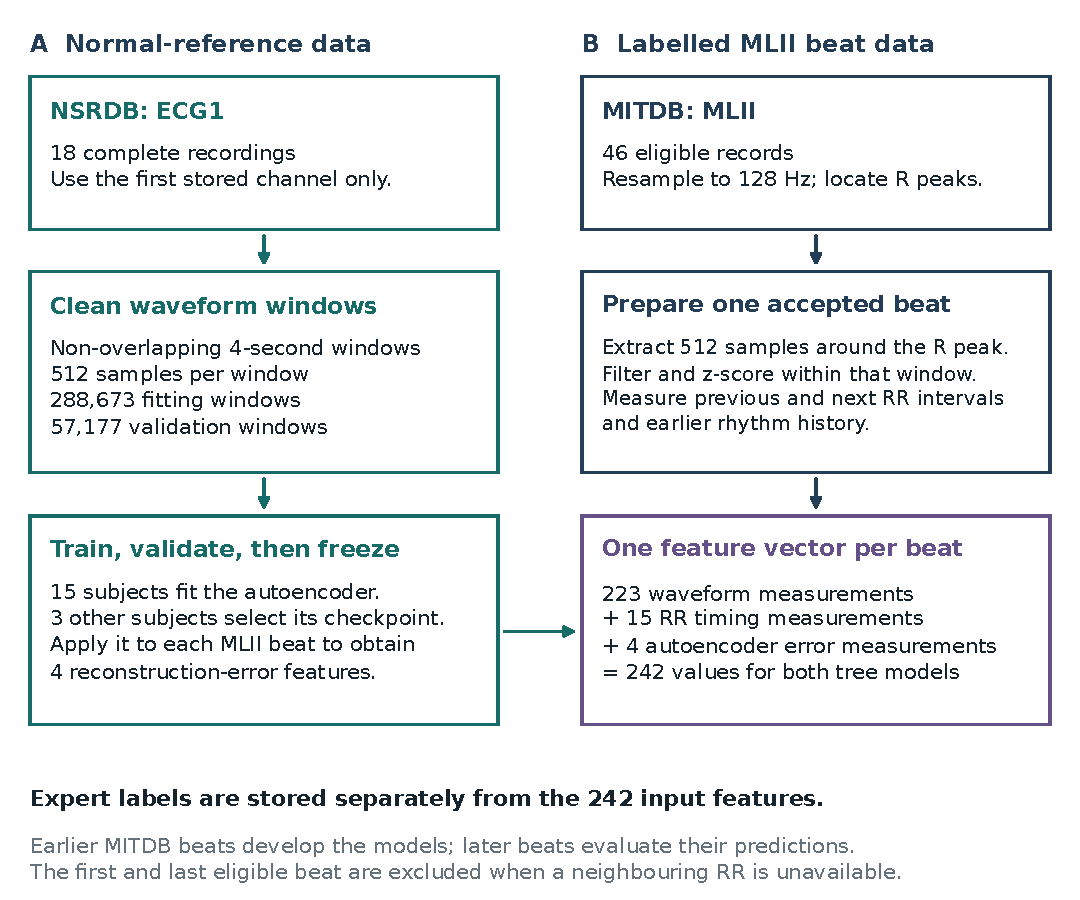
\includegraphics[width=.95\textwidth]{pic/generated/real_data_preparation_flow.pdf}
\caption[Preparation of normal-reference windows and labelled MLII beats.]{Preparation
of normal-reference windows and labelled MLII beats. Panel A develops the frozen
autoencoder from subject-disjoint NSRDB fitting and validation data. Panel B
uses local filtering and standardisation for each MITDB beat, then combines
waveform, RR timing, and frozen-autoencoder residual features. Expert labels
remain separate from the model input.}
\label{fig:data-feed-real}
\end{figure}

\subsubsection{Inputs to the frozen system}

During autoencoder fitting, Gaussian noise with standard deviation 0.03 is
added to each input while the clean NSRDB window remains the target. During
supervised fitting, record-and-class weights reduce domination by long records
and common classes. During prediction, one MLII window, its observed previous and next RR
intervals, and its recent RR history are converted into the same 242-value vector used in the temporal
experiment. A decision of N ends classification for that beat. An abnormal decision passes
the same vector to the subtype model. Section~\ref{ch:theory} explains the theoretical basis of these features and
the two-stage decision. The allocation is evaluated under the protocol in
Section~\ref{ch:method}.
